\documentclass[bsc,frontabs,twoside,singlespacing,parskip,deptreport]{infthesis}
\usepackage{graphicx}
\usepackage{subcaption}
\graphicspath{ {Dissertation/} }
\usepackage{gensymb}
\begin{document}


\title{Designing a System to Quantify Waste in Domestic Heating}

\author{Joel Hutton}

\course{Computer Science and Electronics (BEng Hons) }
\project{{\bf Beng Hons Project Report}}

\date{\today}

\abstract{
The aim of the project is to build a system to quantify waste in domestic heating. Temperature, motion and light are measured by custom built sensors. The sensors are also capable of sniffing WiFi traffic to see what devices are nearby. 
}

\maketitle

\tableofcontents

%\pagenumbering{arabic}


\chapter{Introduction}

Many heating systems in the UK have some ability for automatic control, from basic timer and thermostat to advanced zoned internet connected systems. These systems are only effective if used correctly and if people do not have the time or ability to use them effectively energy is wasted and the residents are not at a comfortable temperature. This system measures temperature, motion and light as well as sniffing WiFi traffic to identify nearby devices. This data is sent to a server for data storage and analysis. Users are periodically asked by text whether they are at a comfortable temperature and what room they are in to collect data on what temperature is comfortable for them and validate occupancy data. The system aims to make the user aware of where and when they are wasting energy by giving temperature graphs annotated with room occupancy and ideal temperature.        

\section{Designing The Hardware}
\subsection{Requirements}
Cost is an important requirement and the target cost per sensor is £10 in parts. As these sensors will be retrofitted wireless communication is essential to avoid the need for running ethernet cables throughout the property. The hardware needed to be able to measure temperature, motion and light. It is desirable to be able to measure humidity and prescence of WiFi devices but not essential.

\subsection{Wireless Communication}
WiFi was the preferred choice of communication as it removes the need for any 'bridge' and utilises existing hardware (the router) and thus reduces cost and means a user can start with a single sensor. It also gives the ability for each sensor to monitor present devices, and possibly determine where the device was with multiple sensors. 

\subsection{Microcontroller}
The microcontroller needs to have enough 
The ESP8266 was chosen as it can be obtained for \$3 in small quantities, has WiFi built in, good community support and has hotspot capability, as it could be useful for configuration. It also has an analogue to digital converter (ADC) which is useful for measuring analogue sensors. 

\subsection{Temperature sensor}
The DHT22 was initially selected as it was a combined temperature and humidity sensor, for low cost \$2.5/unit at low quantities. r. 

\subsection{Circuit Design}
The circuit was prototyped on a solderless breadboard, to test the software and hardware. The initial circuit can be seen in Figure \ref{breadboard}. 
\begin{figure}[ht]
\label{breadboard}
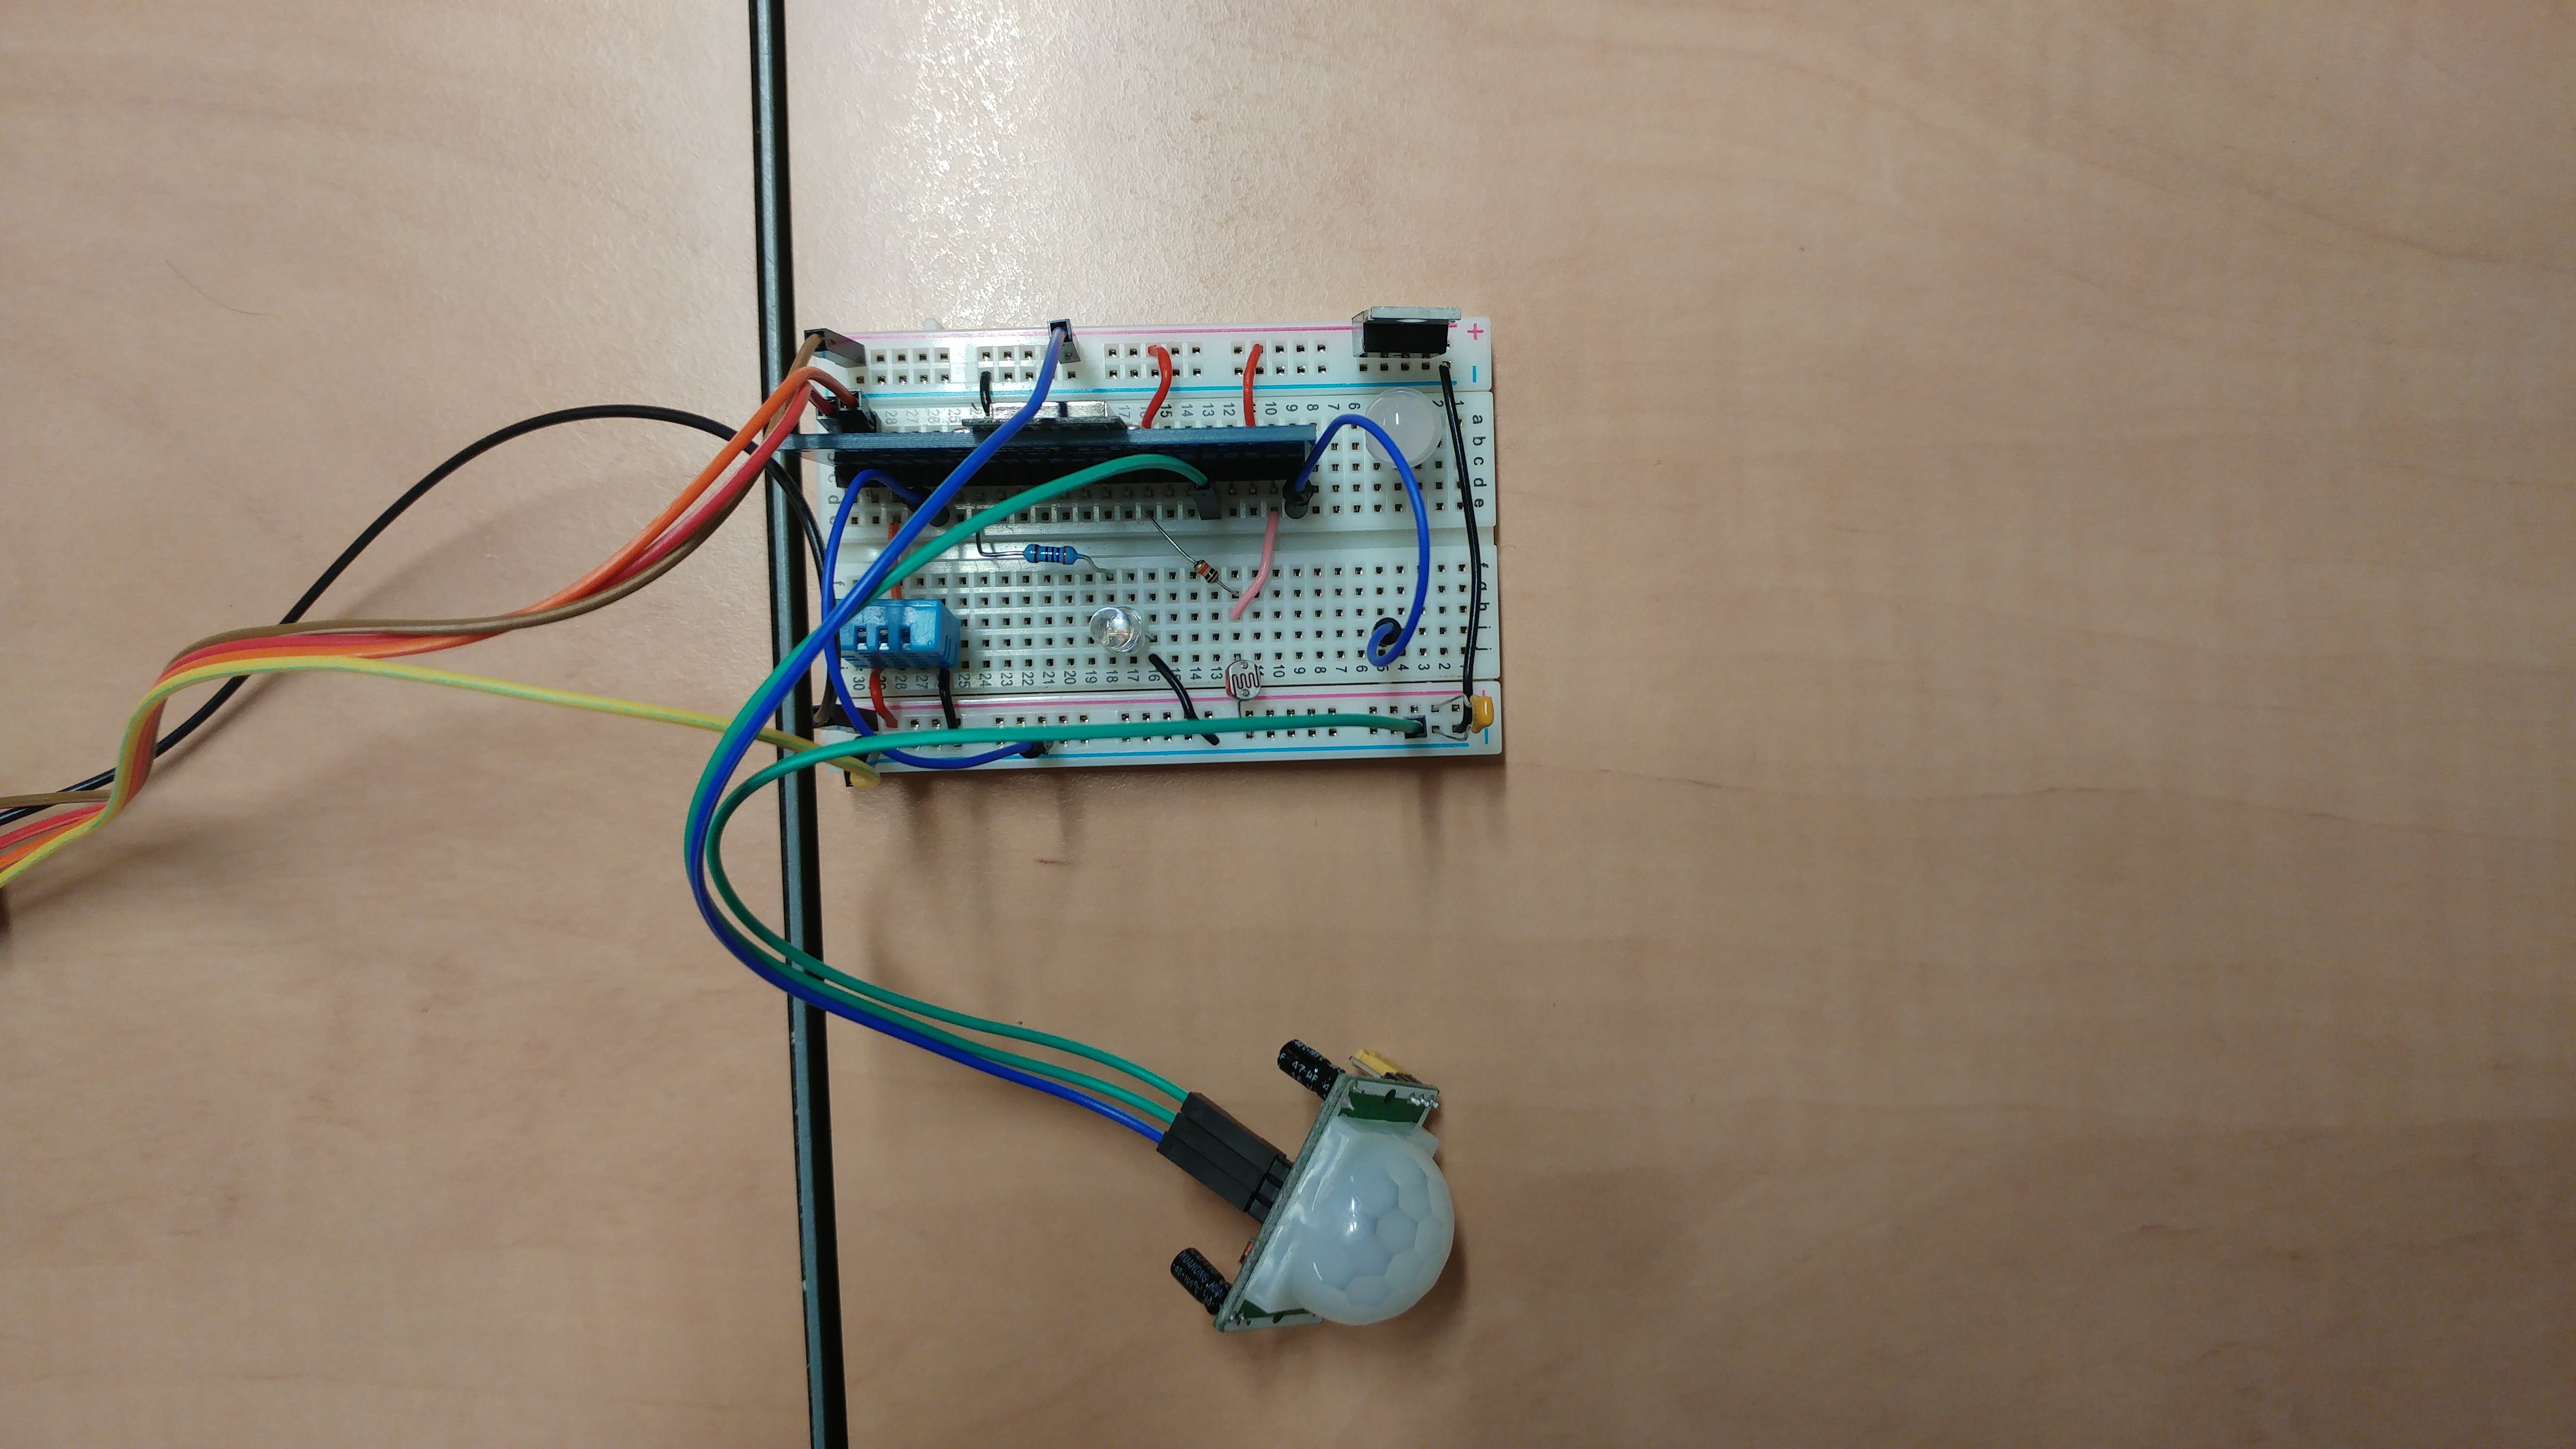
\includegraphics[scale=0.08]{20161130_162235.jpg} 
\caption{Prototype Circuit}
\end{figure}

\begin{center}
\begin{figure}[ht]
\label{initial}
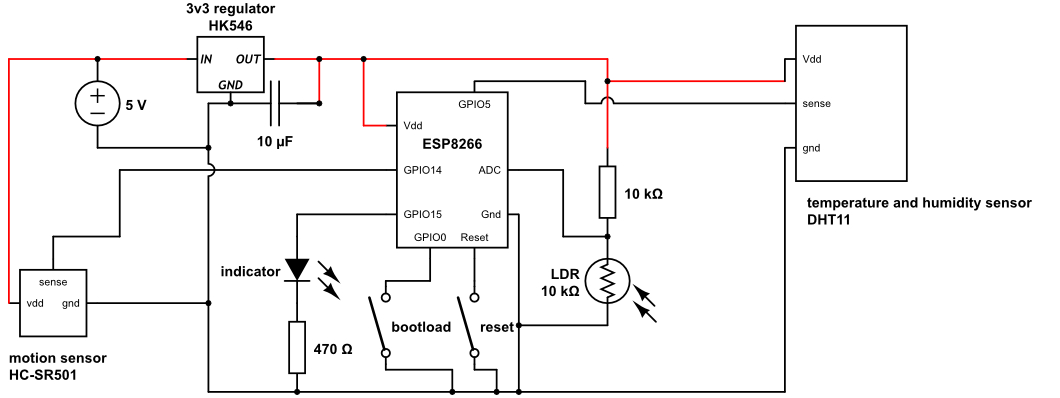
\includegraphics[scale=0.6]{initial_circuit.png} 
\caption{Prototype Circuit Diagram}
\end{figure}
\end{center}

\subsection{Improvements to Circuit}
The circuit was tested by leaving it overnight in a kitchen transmitting to a server while the room was in normal use. Upon graphing the temperatures seen overnight 2 problems became evident, the temperatures were being treated as integers, and the temperature sensor was far out of spec. The first problem was evident by points only appearing on whole number values, the second evident as the temperature varied rapidly within a 5\degree C range. The temperature sensor was replaced by another DHT22 but the inaccuracy persisted.

After testing showed very poor performance for the DHT22 with temperatures far out of spec, the sensors disagreed on temperature and gave inconsistent readings. The ds18b20 was chosen as a replacement as it could take the same place as the DHT22. Both sensors have 3 used pins Vdd, data, gnd in that order, making the ds18b20 a drop in replacement in hardware, along with some software changes as it uses a different protocol. A 1k pull up resistor was added in accordance with the documentation for the ds18b20. 

Another change was using an ESP8266 based dev board - the Wemos D1 mini - instead of the chip itself. This integrated the voltage regulator, bootloader and reset buttons and cost the same as the ESP8266 making it a cost saving when the voltage regulator and buttons are considered. The D1 also had a micro usb connector for convenient power supply and programming compared to soldering directly to the board.

After finalising the circuit it was moved onto veroboard.
The layout was drawn out on squared paper before being copied onto the top and bottom of the veroboard. board breaks on the veroboard Figure \ref{veroboard}. 

Considerations for the layout included:
\begin{itemize}
\item having trace antenna overhanging the board so that capacitance with the copper cladding does not interfere and attenuate the signal
\item keeping temperature sensor far away from sources of heat such as the D1
\item keeping button accessible
\item keeping led and light sensor apart so the led does not affect the light readings
\item reducing the number of wires needed by using the rails effectively
\item reducing the number of breaks needed between holes as these are laborious
\item keeping the area of the board down to keep the sensors small \\
\end{itemize}
The final circuit required only one break between holes and kept the board relatively compact. 

\begin{figure}[ht]
\begin{subfigure}{.5\textwidth}
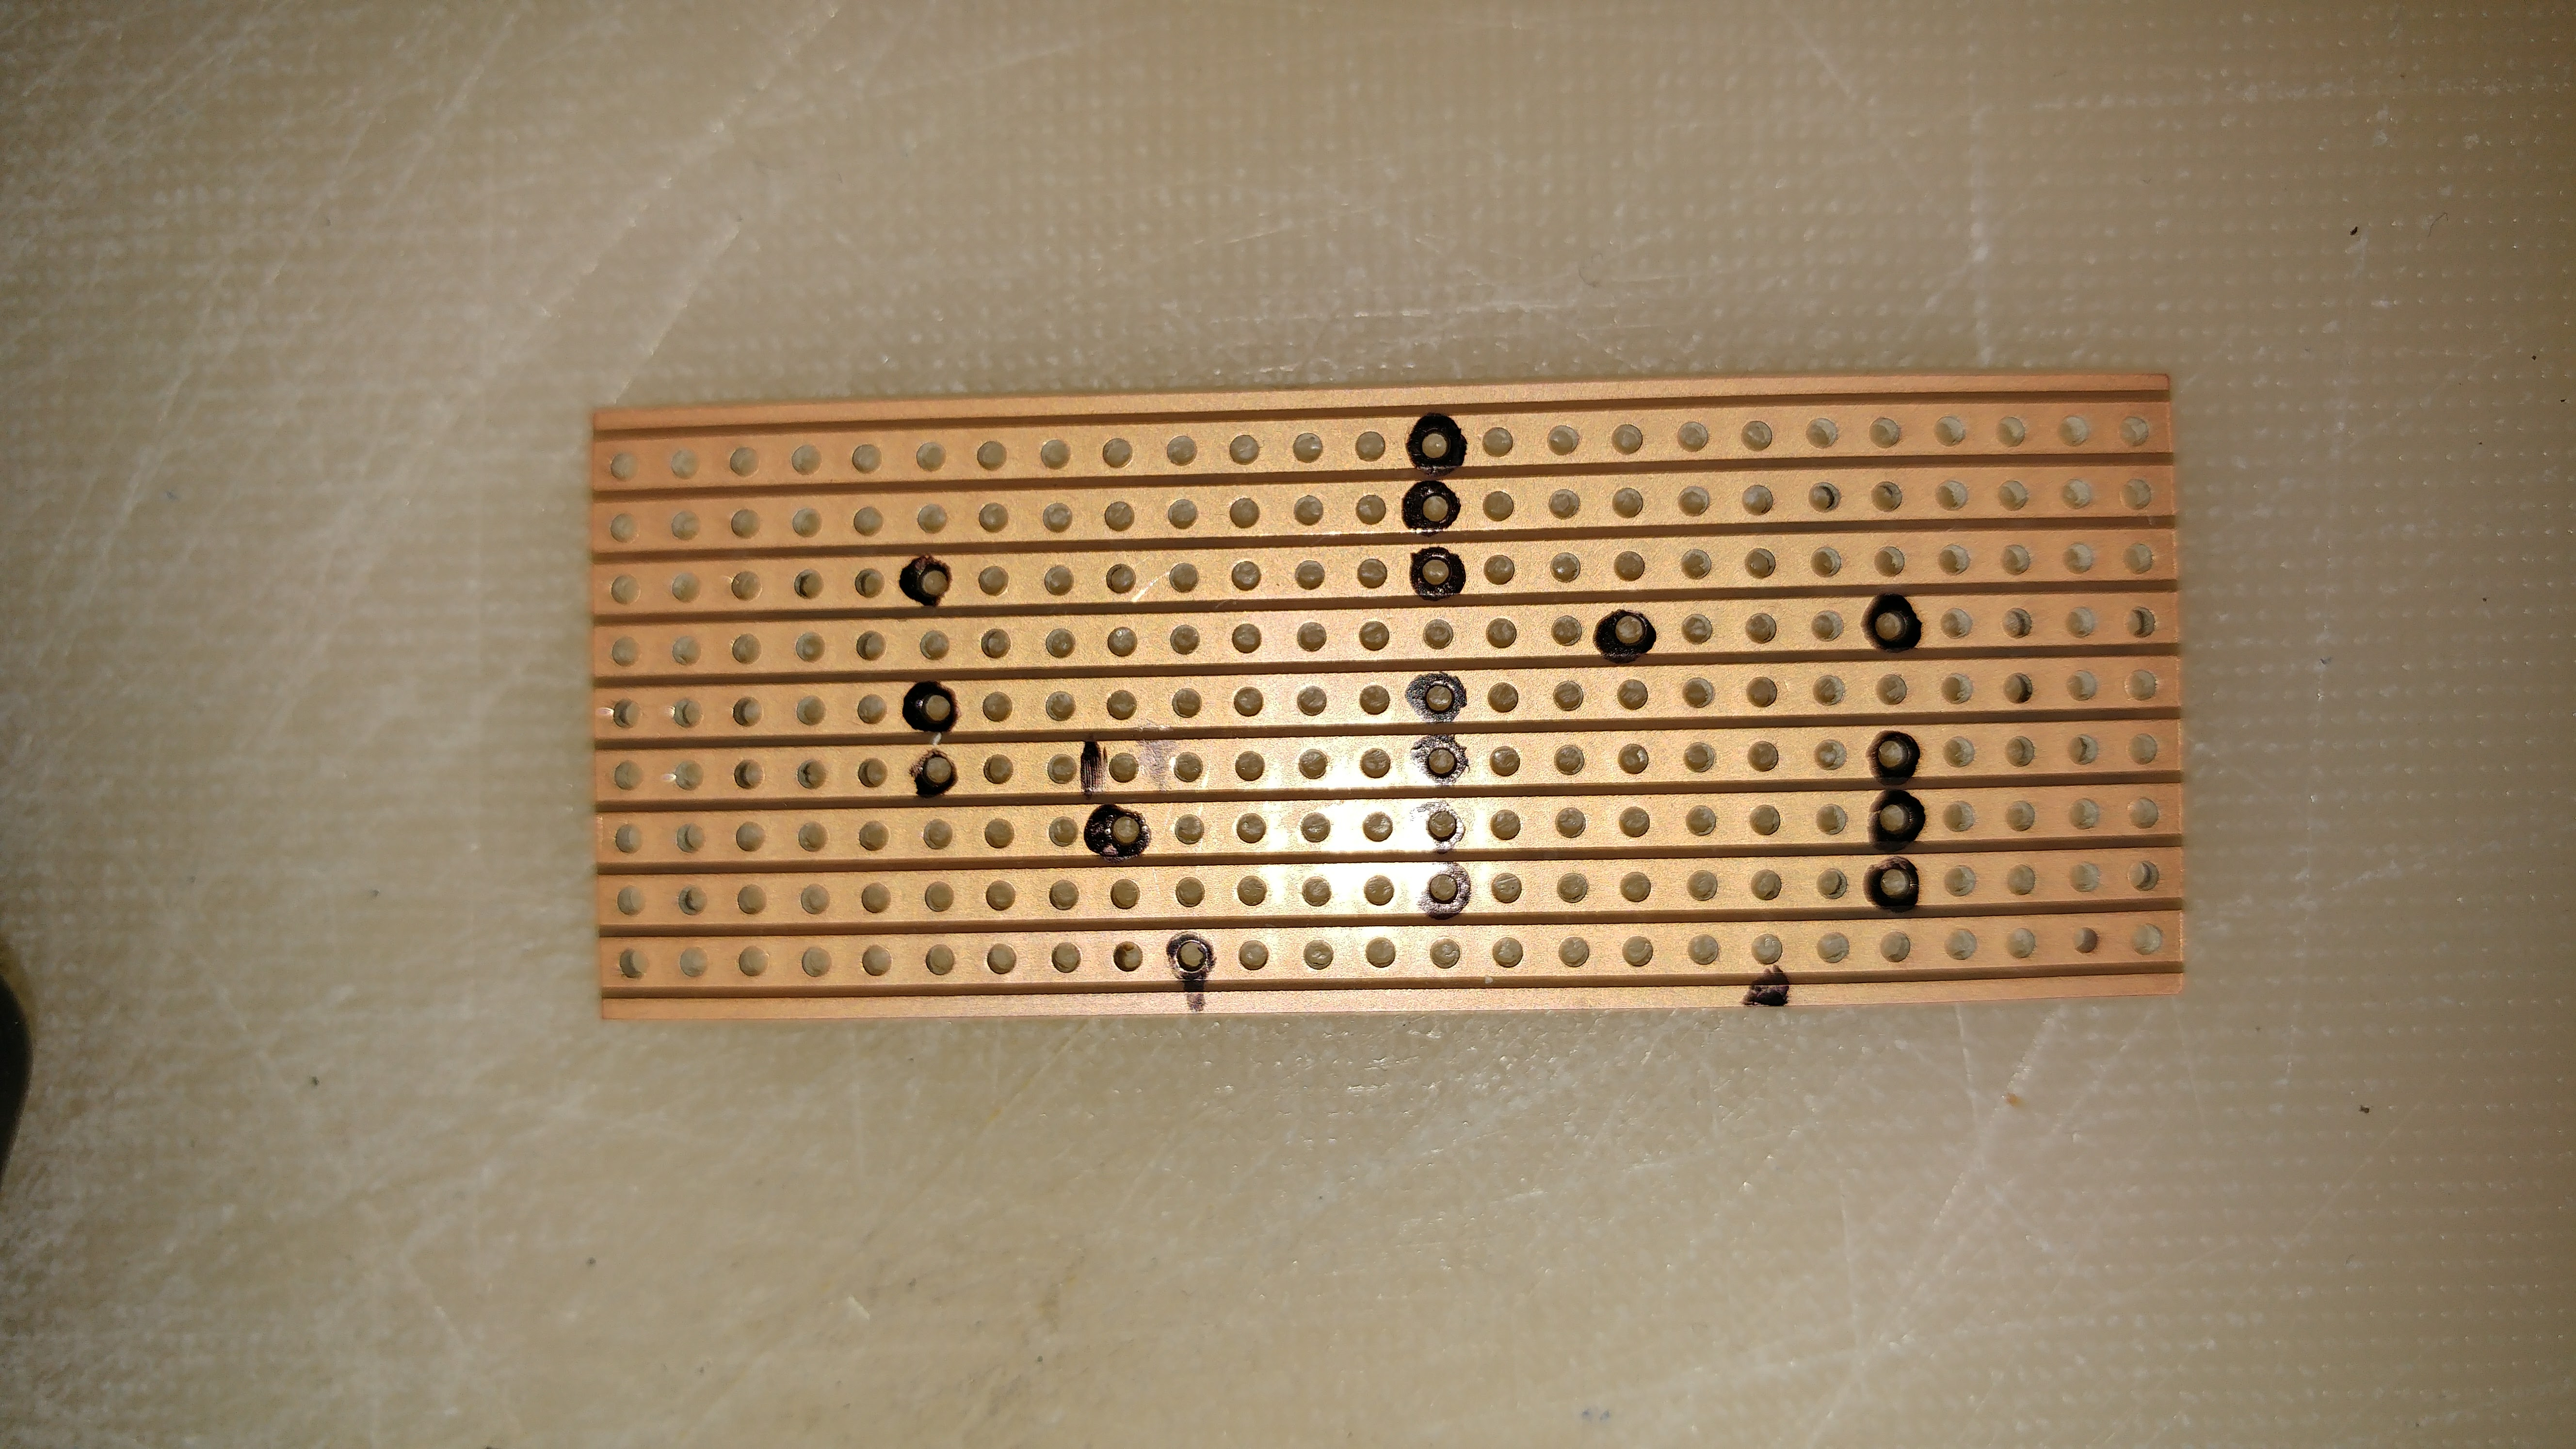
\includegraphics[width=.8\linewidth]{20161230_150858.jpg} 
\caption{Underside with copper cladding}
\end{subfigure}
\begin{subfigure}{.5\textwidth}
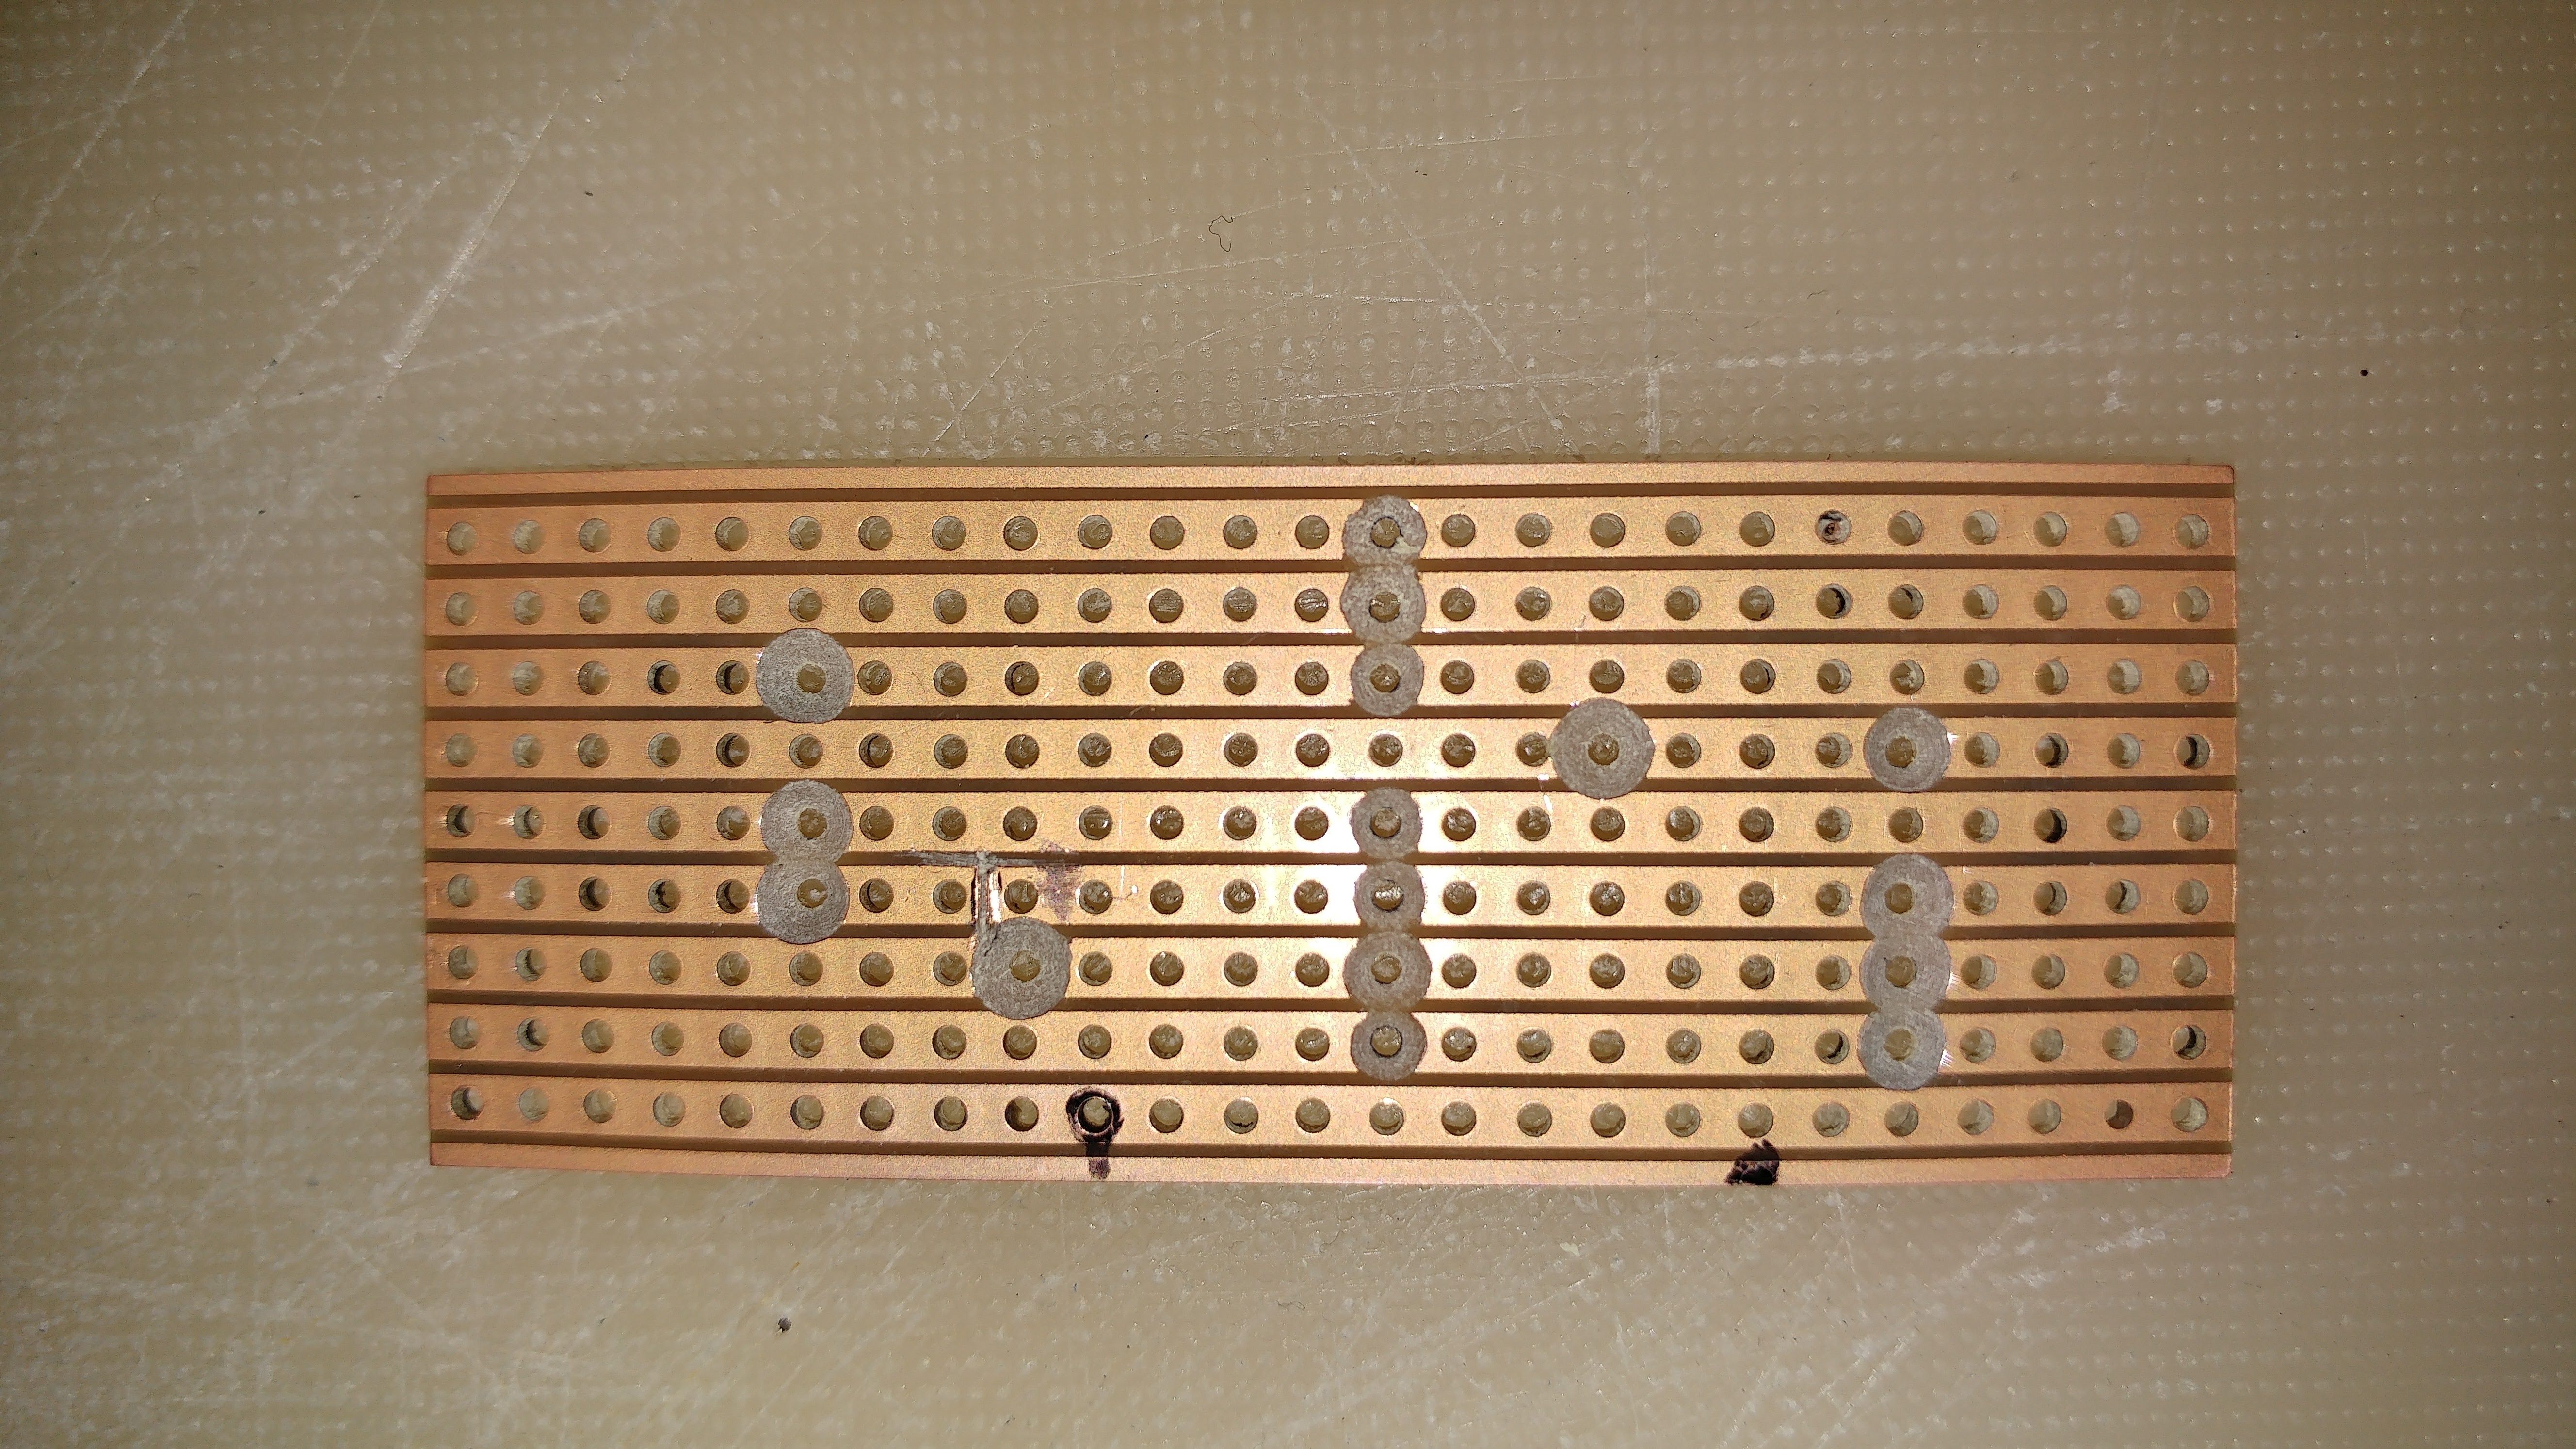
\includegraphics[width=.8\linewidth]{20161230_151405.jpg}
\caption{Underside with breaks drilled}
\end{subfigure}

\begin{subfigure}{.5\textwidth}
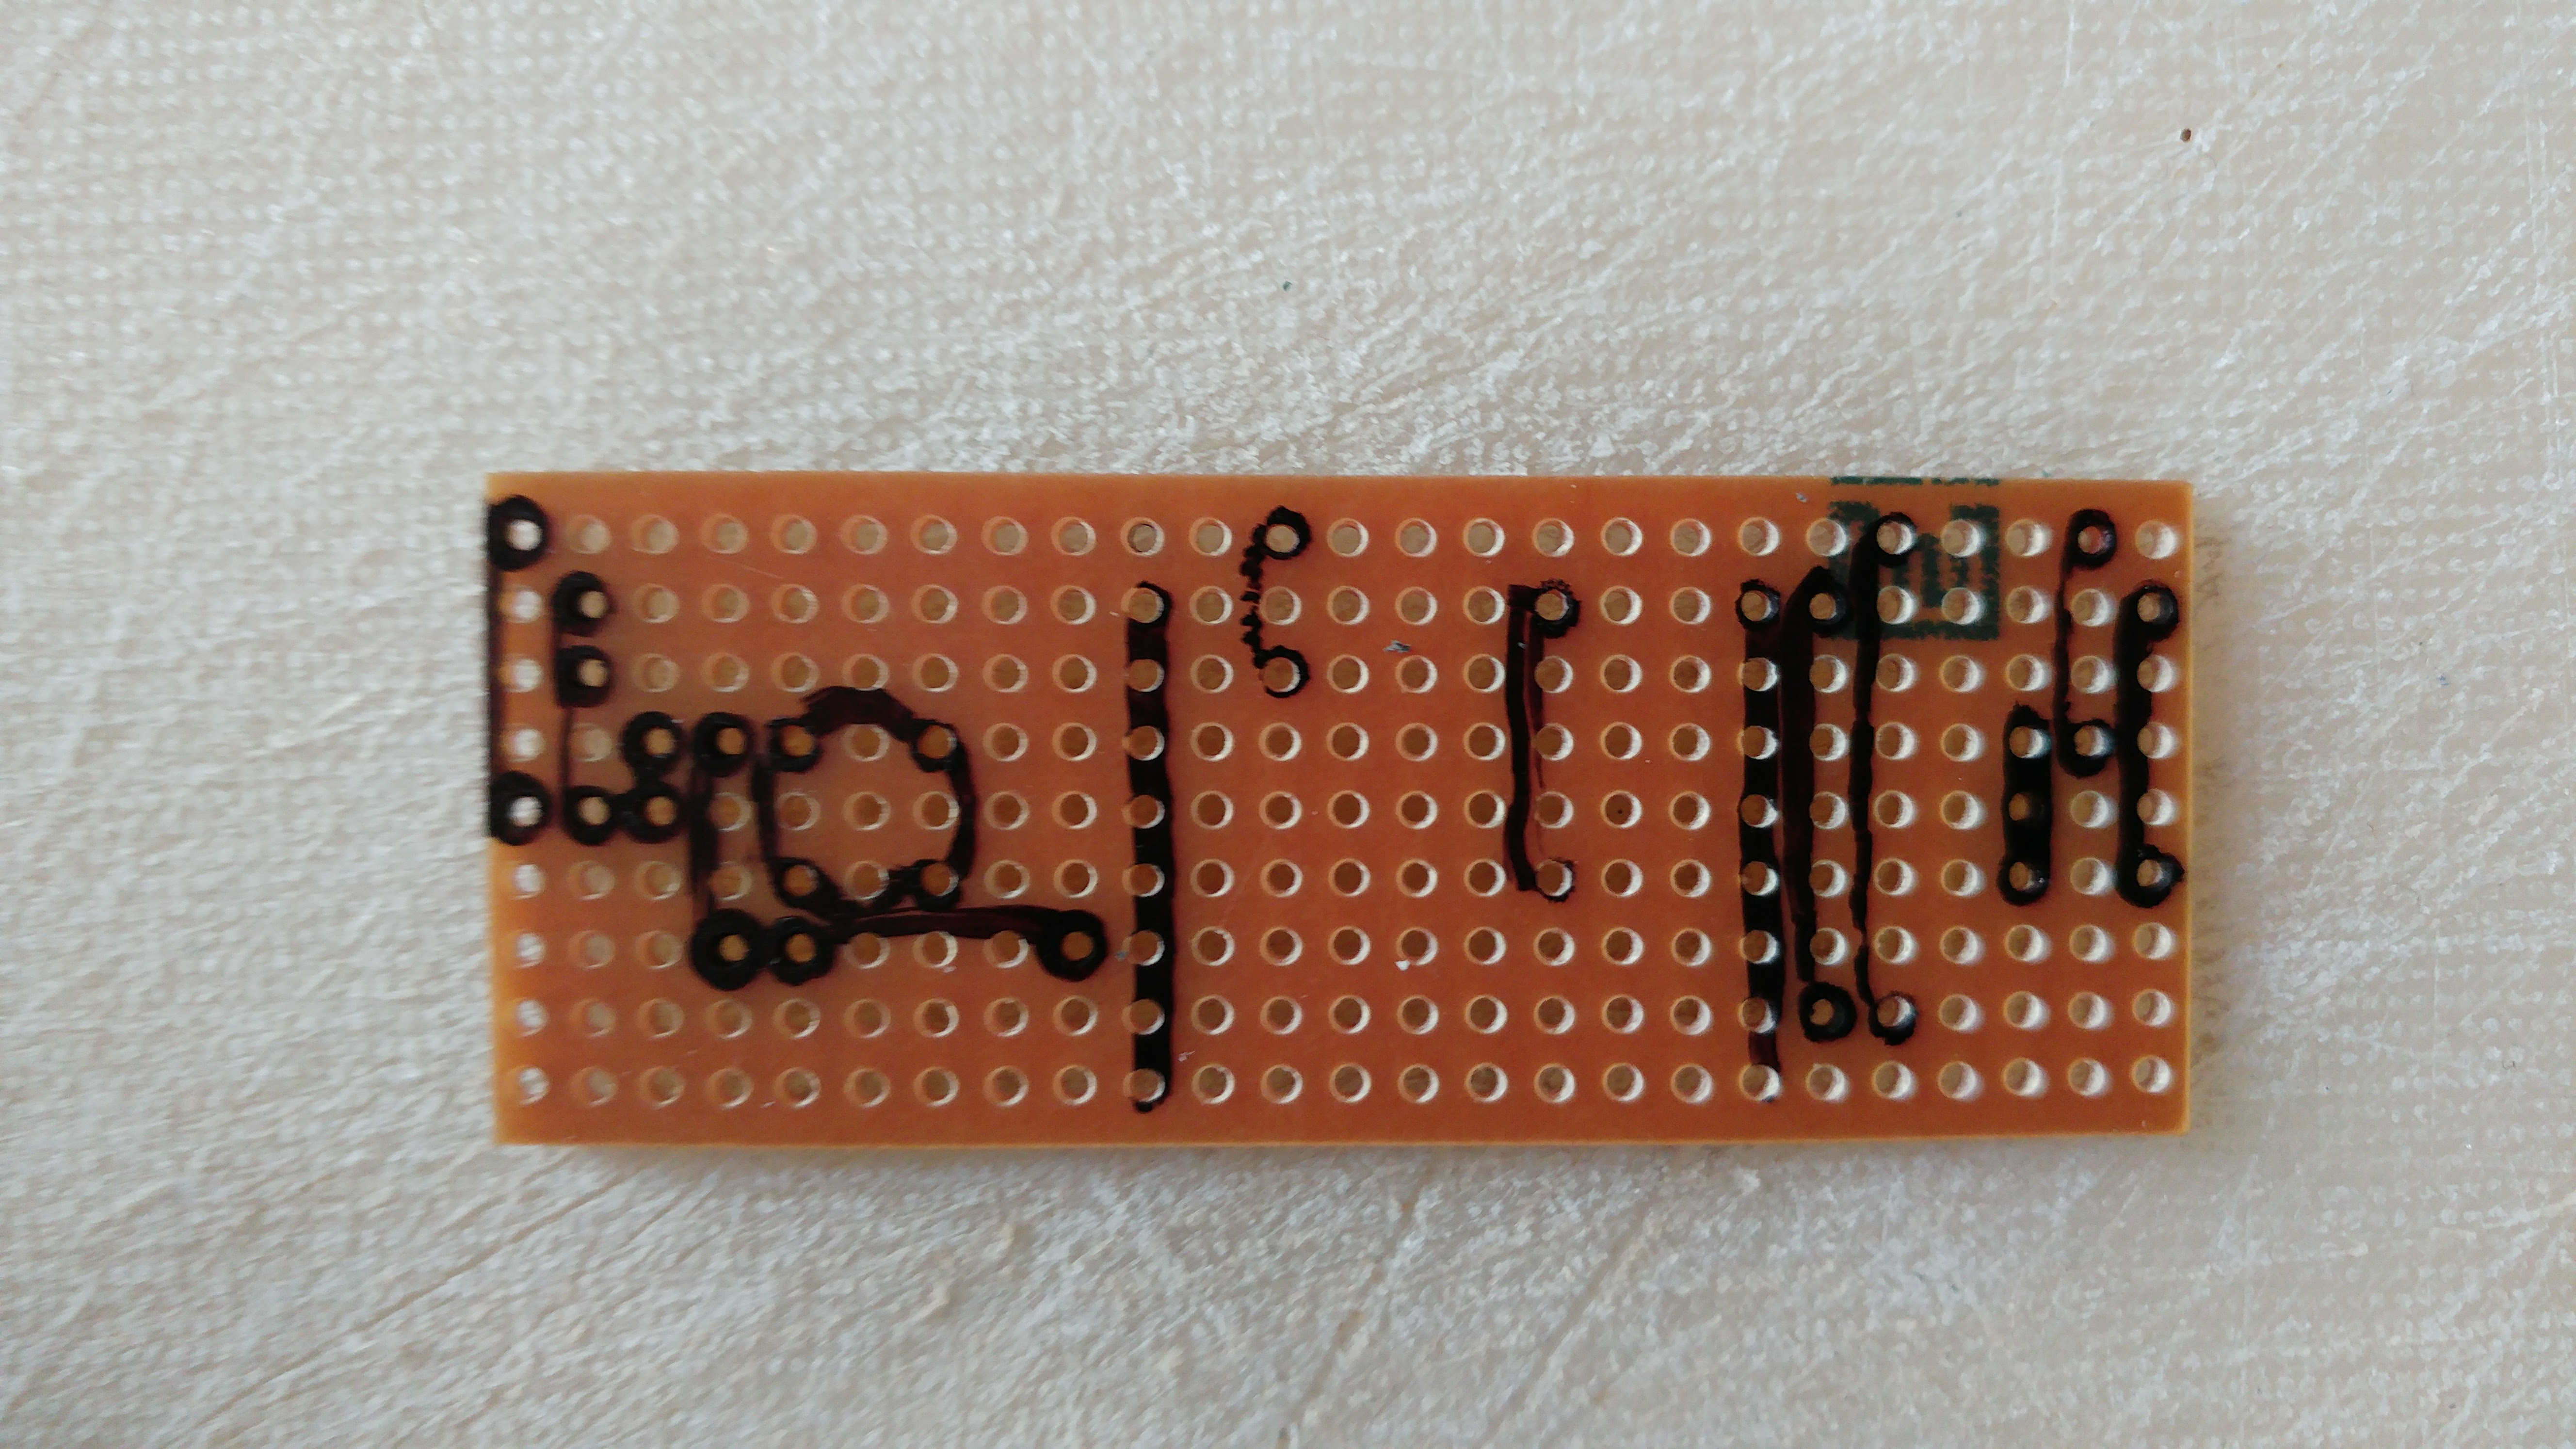
\includegraphics[width=.8\linewidth]{20161230_143726.jpg} 
\caption{Upperside with Components marked out }
\end{subfigure}
\begin{subfigure}{.5\textwidth}
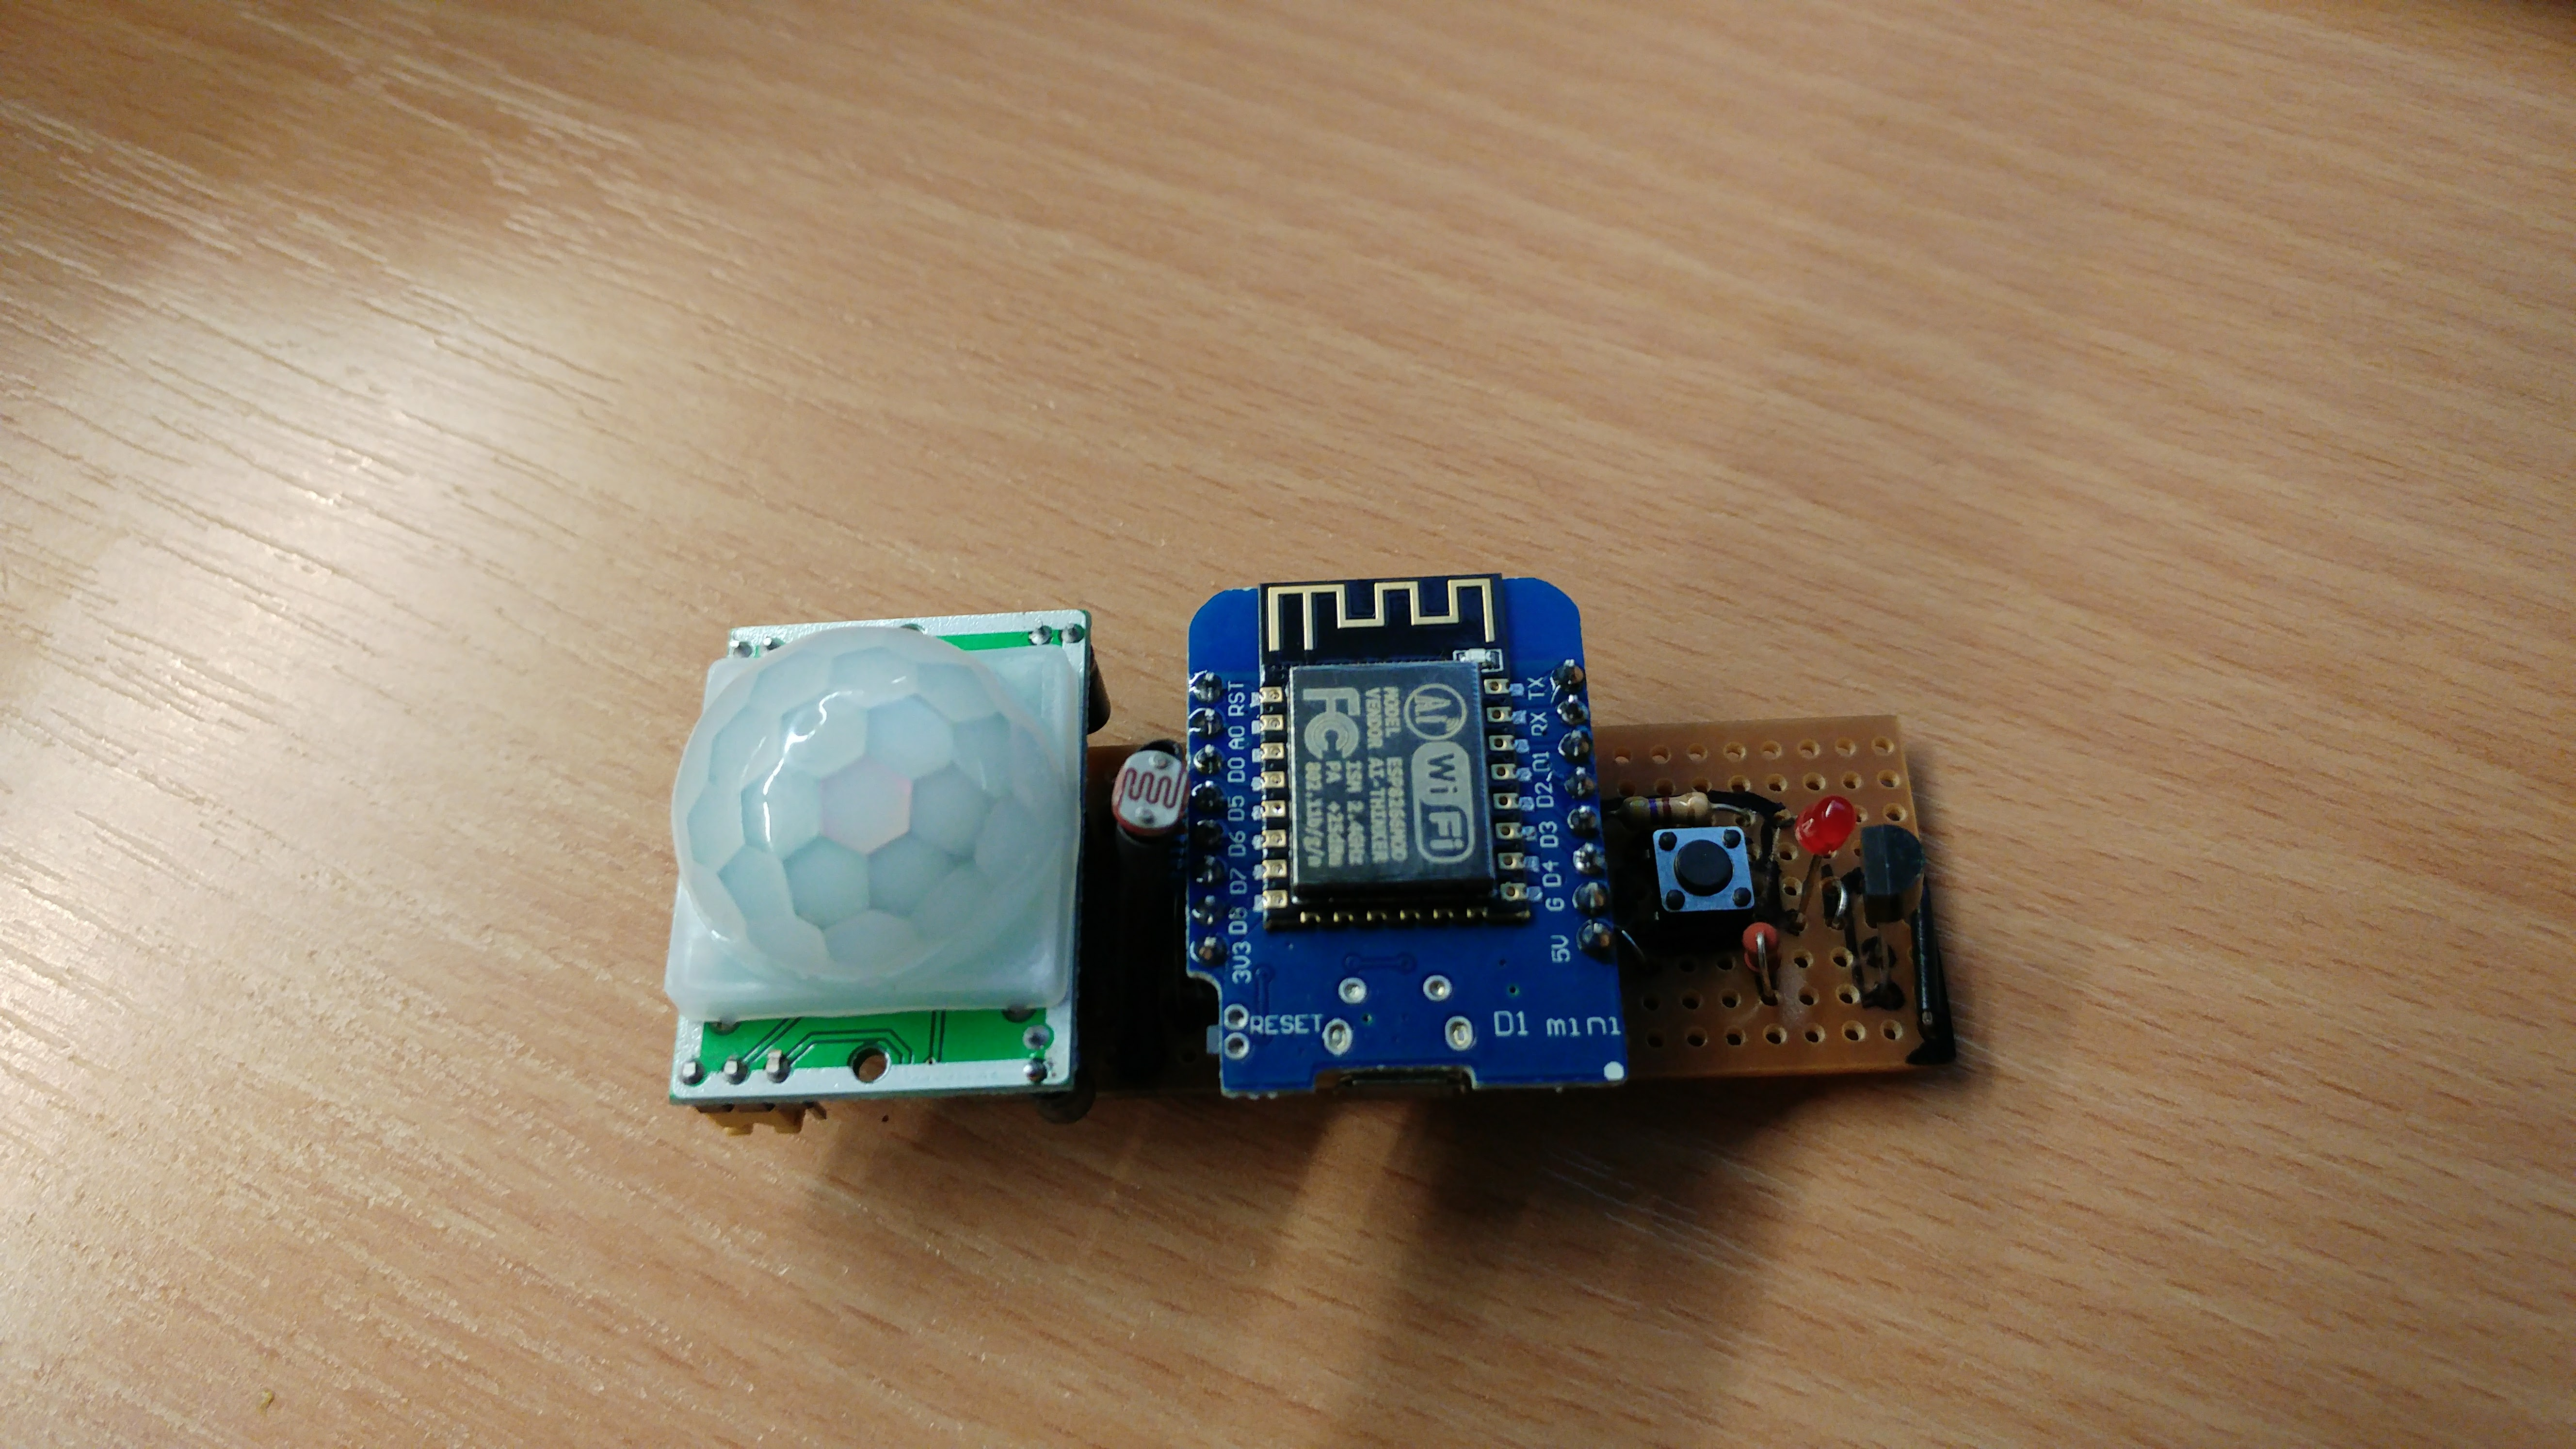
\includegraphics[width=.8\linewidth]{20170125_181446.jpg} 
\caption{Upperside with Components placed }
\end{subfigure}
\end{figure}

\begin{figure}
\begin{center}
\centering
\label{final circuit}
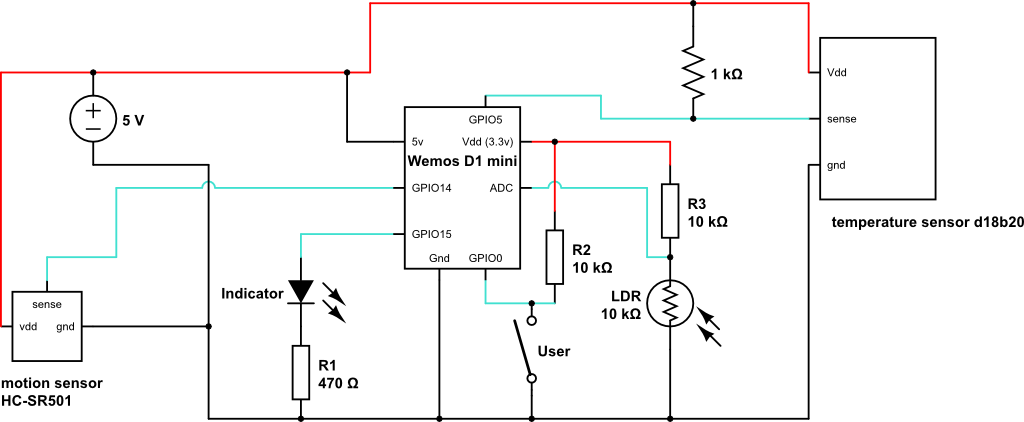
\includegraphics[scale=0.6]{dissertation.png}
\caption{Revised circuit with colour coding}
\end{center}
\end{figure}
Testing showed the board performed as expected and the rest of the boards were made to the same design. 

\subsection{Fabricating the Sensors}
Once the prototype was tested the remaining 14 sensors were made in stages, labelling all the boards from 2-15, marking the undersides of the boards, marking the uppersides of the boards, drilling out the copper traces with an electric drill (a hand tool is normally used but due to the relatively high volume a drill was faster), testing all the traces had been cut with a voltmeter, placing components, then soldering components. As 15 boards needed to be tested so a test program was written to test each feature - first blinking the led, then giving light readings and requesting the user to cover the light sensor, giving motion readings and requesting the user to move, finally giving temperature readings and requesting the user to pinch the temperature sensor in between their fingers. The tests which could not be passed were recorded for each sensor in a spreadsheet along with the solution when it was fixed, some mistakes were identified and fixed. 

\section{The Server}
\subsection{The Database}
A sqlite database was created to store the information from the sensors. The initial design is as shown in Figure \ref{sqlinitial} 

\subsection{The Daemon}
A daemon was written to receive packets from the sensors and put it into a database. Packets received from unregistered sensors are ignored and a record is placed into the unregistered sensors table (not shown). A management program allows registration of sensors into the database. 

\section{Still to Do}

\begin{itemize}
	\item complete data collection
	\item analyse data 
	\item complete write up
\end{itemize}

\begin{figure}
\begin{center}
\centering
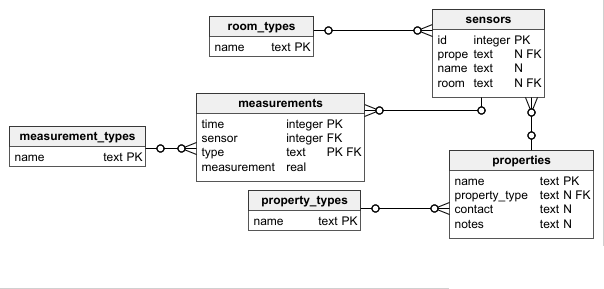
\includegraphics[scale=0.6]{initial_db.png}
\caption{\label{sqlinitial}Initial database design}
\end{center}
\end{figure}

\end{document}